\subsection{Calculation of water height to propagate}
The first step consists in computing the water quantity at the top of the SU. This value is calculated using the following equation if the variable exfiltration is previously produced.

\begin{equation}
\label{height}
H = R + \left(\frac{Q_e\times \Delta t}{A}\right)
\end{equation}


where $H$ is the water height at the soil surface ($m$), $R$ is the runoff water height ($m$) generated by the production function, $Q_e$ is the exfiltration discharge ($m\up3/s$), $A$ is the surface of the SU ($m\up2$) and $\Delta t$ is the simulation time step ($s$).\\

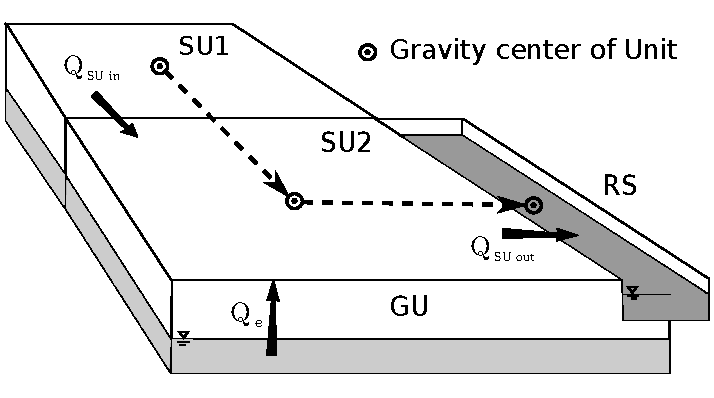
\includegraphics[width=8cm]{doc/common/Schema_GU_RS_SU_Hayami_SU.pdf}

The exfiltration discharge $Q_e$ could be produced by the simulator ``Interflow''.\\


\subsection{Propagation using Hayami kernel}
Then, the water height previously calculated is propagated between the gravity center of the main SU and the downstream unit. The downstream surface unit could be an other SU or a reach segment RS according to the topology. Thus, the calculation is done following the Straler order, from upper SU to downstream SU and RS.\\

The propagation is done using the diffusive wave model :

\begin{equation}
\frac{\delta Q}{\delta t} = -C \times \frac{\delta Q}{\delta x} + D \delta \frac{\delta \up2 Q}{\delta x\up2}
\end{equation}




Celerity and diffusivity are considered as time constants to simplify the equation and resolved it using the Hayami analytical method \cite{Moussa1996}. The model consists to convolute the input water height by using the following equation :

\begin{equation}
\begin{array}{l}
Q_{SU}(t) = \frac{d}{2\times (\pi \times D)\up{1/2}} \times exp ^{\frac{C \times d}{2 \times D}}
\\
\ \ \ \ \ \ \ \ \times \int_0^t H(t-\tau)\times A \times \frac{ exp ^{\frac{C\times d \times}{4\times D} \times \left(\frac{d}{C \times \tau} + \frac{C \times \tau}{d} \right)}}{\tau \up{3/2}} \delta \tau
\end{array}
\end{equation}




where $Q(t)$ is the produced water discharge at time $t$ ($m\up3/s$), $d$ is the distance between the gravity center of the two connected units ($m$), $D$ is the wave diffusivity ($m\up2/s$), $C$ is the wave celerity ($m/s$), and $A$ is the surface of the SU ($m\up2$).\\

The term $H(t-\tau)$ is the water height at the soil surface calculated in equation \ref{height}. This water height is convoluted with the ``Hayami kernel'' $K(t)$ which is given as :

\begin{equation}
K(t) = \frac{d}{2 \times (\pi D)^{\frac{1}{2}}} \times \frac{\text{exp}^{\frac{Cd}{4D} \times \left(2-\frac{d}{Ct}- \frac{Ct}{d} \right) } }{t^{\frac{3}{2}}}
\end{equation}




The convolution operation is schematized below :

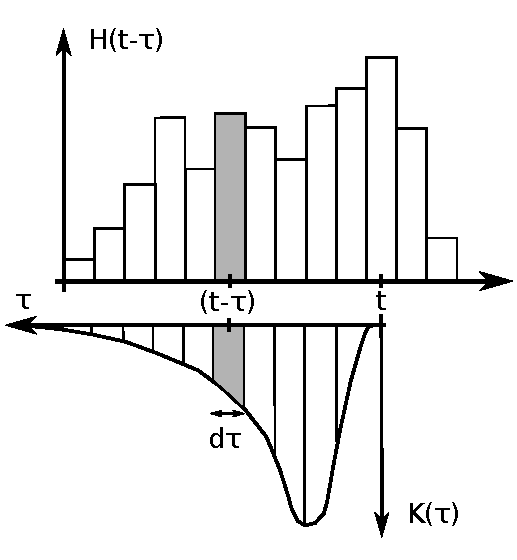
\includegraphics[width=8cm]{doc/common/Convolution_HayamiSU.pdf}

$\tau$ is an operator of the convolution product which is internal to the simulator. To do this, the simulator temporarily sweeps the Hayami kernel, at the simulation time step $\delta \tau$, up to a maximum step defined as $MaxSteps$ parameter ($-$). So, the duration of Hayami kernel is equal to $MaxSteps.\Delta t$. Consequently, this parameter should be ajusted according to the kernel shape and the simulation time step. The higher this parameter is, the better the difinition of Hayami kernel is, but the longer the simlation is. Moreover, the smaller the simulation time step is, the better the Hayami kernel resolution is. To optimize the parametrization for a given simulation time step, the better way is to set a high value of $MaxSteps$ and decreases it while the results doesn't change.\\

The two main parameters $C$ and $D$ of the diffusive model could be related to the slope and the rugosity of the surface unit using Manning-Strickler relation.

\begin{equation}
C=C_u\times \sqrt{\frac{\beta}{\beta_m}}\times \frac{n_m}{n} \ \ \ \ \ et \ \ \ \ \ D=D_u\times \frac{\beta}{\beta_m} \times \frac{n_m}{n}
\end{equation}


where $C_u$ is the mean celerity of SUs ($m/s$), $\beta$ is the slope of the SU on which the calculation is done ($m/m$), $\beta_m$ is the mean slope of SUs ($m/m$), $n$ is the rugosity coefficient of the SU ($s/m\up{1/3}$), $n_m$ is the mean rugosity coefficient of SUs ($s/m\up{1/3}$) and $D_u$ is the mean diffusivity of SUs ($m\up2/s$). This calculation is done only once at the beginning of the simulation.\\

Both parameters determine the Hayami unit hydrogram shape. The following figure shows different shape of hydrogram as a function of $w$ and $z$ parameters which are expressed hereafter :

\begin{equation}
w = \frac{L}{D} \ \ \ \ \ z = \frac{C.L}{4.D}
\end{equation}



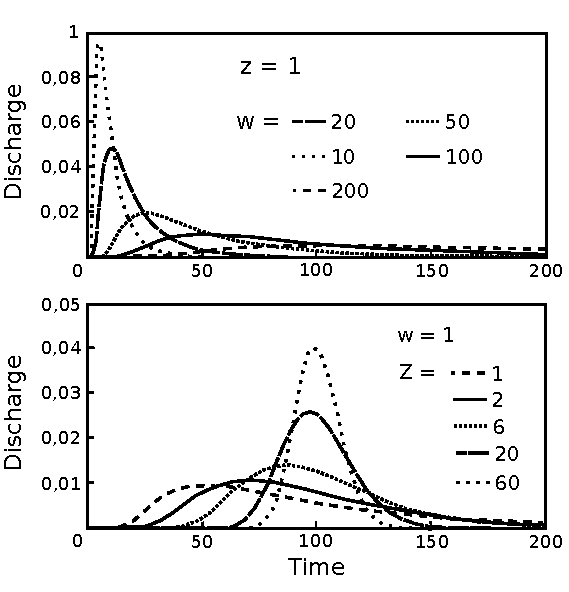
\includegraphics[width=8cm]{doc/common/Graphique_noyau_Hayami.pdf}

Examples of use and parametrization are available in the thesis of Chahinian \cite{Chahinian2004} and the paper of Moussa and al. \cite{Moussa2002}.\\
